\section{Modello del paziente}
L'organismo umano è un sistema molto complesso, formato da molti sottosistemi interagenti fra loro e altrettanto complessi, come ad esempio il sistema cardio-circolatorio, nervoso, respiratorio, digerente, \ldots
La dialisi è una procedura terapeutica che serve a ristabilire, per quanto possibile, un equilibrio chimico e volumetrico dell'organismo e, per questo motivo, verrà considerata solo quella parte dell'organismo direttamente coinvolta negli scambi di liquidi e soluti, ignorando tutto il resto.

Quello che è racchiuso in \figurename~\ref{schema_generale} dalla linea tratteggiata grigia e recante l'etichetta ``\textsc{Paziente}'' rappresenta ciò che può essere considerato il paziente nel contesto dialitico: si tratta di un recipiente, formato da tre compartimenti sempre più profondi e capienti, separati da due membrane semipermeabili: la membrana capillare e la membrana cellulare. Questo schema è tratto da Guyton et al. \cite{guyton}. Nella realtà fisiologica, tuttavia, non esistono compartimenti e membrane così ben definiti. Nell'organismo umano infatti le cellule, e ciò che racchiudono, sono distribuite in maniera omogenea in tutto il volume corporeo; lo spazio interstiziale è un ambiente identificato topologicamente dal percorso che i metaboliti compiono per passare dall'apparato circolatorio alle cellule; il volume plasmatico è contenuto nelle arterie, vene e capillari dell'organismo. Per le membrane cellulari e capillari il discorso è analogo: esistono numerose membrane di ambo i tipi sparse omogeneamente all'interno del volume corporeo. Per agevolare la trattazione matematica si è deciso di semplificare il problema andando a ``concentrare'' i volumi cellulari, interstiziali ed ematici distribuiti nell'organismo, in tre compartimenti nettamente separati dalle membrane appropriate. Questa semplificazione risulta essere una pratica ampiamente consolidata nella modellizzazione del paziente sottoposto a dialisi \cite{casagrande, gatti, ursino}.

\subsection{Bilancio di massa nel compartimento intra-cellulare}
L'equazione che descrive il bilancio di massa per uno specifico soluto, all'interno del compartimento intracellulare è:
\begin{equation}
	\frac{dM_{ic}}{dt} = G_{ic}+ \Phi_{ic}
	\label{eq:dMic}
\end{equation}
dove:
\begin{itemize}
	\item $G_{ic}$ è il tasso di generazione del soluto all'interno delle cellule;
	\item $\Phi_{ic}$ è il flusso di massa del soluto verso l'interno del compartimente intracellulare.
\end{itemize}
\begin{figure}[htb]
	\centering
		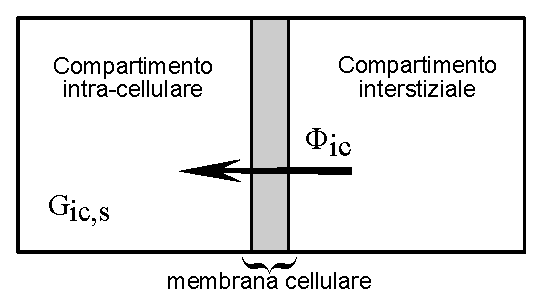
\includegraphics[width=0.5\textwidth]{immagini/massa_ic.eps}
				\caption{Scambio di massa fra compartimento intra-cellulare e interstiziale.}
\end{figure}
La formula per $\Phi_{ic}$ è data dall'Eq.~(\ref{flusso_ic}) e cioè:
\begin{equation}
	\Phi_{ic} = - k \bigl(C_{ic} - \beta C_{is}\bigr)
	\label{eq:phi_ic}
\end{equation}
in cui, come già spiegato in \textsection\ref{trasp_cel}:
\begin{itemize}
	\item $k$ è il coefficiente di trasferimento di massa del soluto attraverso la membrana cellulare;
	\item $\beta$ è il rapporto all'equilibrio fra concentrazione intracellulare e interstiziale del soluto.
\end{itemize}
La concentrazione di un soluto può essere espressa in funzione della quantità e del volume in cui è distribuito. Per il compartimento intracellulare vale ovviamente:
\begin{equation}\label{eq:ovvia}
	C_{ic} = \frac{M_{ic}}{V_{ic}}
\end{equation}
Se si considera l'effetto Donnan (\textsection~\ref{sec:donnan}), si può scrivere la concentrazione interstiziale in funzione di quella plasmatica, ovvero:
\begin{equation}
	C_{is} = \alpha_d\cdot C_{pl}
	\label{eq:donnfrac}
\end{equation}
in cui $\alpha_d$ è il coefficiente di Donnan, specifico per ogni soluto, il cui calcolo è esposto in Appendice~\ref{app:A}.
Ora, poiché il compartimento extracellulare è formato dal compartimento interstiziale più quello plasmatico, per la conservazione della massa vale che:
\begin{align*}
	M_{ex} &= M_{is} + M_{pl} \\
	             &= C_{is} V_{is} + C_{pl} V_{pl}
\end{align*}
e considerando l'Eq.~(\ref{eq:donnfrac}) è possibile scrivere:
\begin{equation}\label{eq:meno_ovvia}
	M_{ex} = C_{is} V_{is} + \frac{C_{is}}{\alpha_d} V_{pl}
\end{equation}
da cui si ricava:
\begin{equation*}
	C_{is} = \frac{M_{ex}}{V_{is} + V_{pl}/\alpha_d}
\end{equation*}
A questo punto, considerando nullo il tasso di generazione intracellulare\footnote{è possibile fare questa semplificazione perché la dinamica di generazione di qualsiasi soluto è molto lenta rispetto alla dinamica degli scambi indotta dalla dialisi.}, si può riscrivere l'Eq.~(\ref{eq:dMic}) nel seguente modo:
\begin{equation}\label{eq:dmic}
	\frac{dM_{ic}}{dt} = - k \biggl(\frac{M_{ic}}{V_{ic}} - \beta \frac{M_{ex}}{V_{is} + V_{pl}/\alpha_d}\biggr)
\end{equation}

\subsection{Bilancio di massa nel compartimento extra-cellulare}
Il bilancio di massa nel compartimento extra-cellulare tiene conto degli scambi di massa attraverso la membrana dei capillari e attraverso la membrana del dializzatore e si tratta, per convenzione, di flussi in uscita e quindi negativi; in formule:
\begin{equation}
	\frac{dM_{ex}}{dt} = -\Phi_{ic} -\Phi_{hdf} + Q_s\cdot C_s
\end{equation}
in cui:
\begin{itemize}
	\item $Q_s$ è la portata del fluido di sostituzione (ovvero la portata di pre- o post-diluizione), letta sul monitor della macchina;
	\item $C_s$ è la concentrazione del soluto nel liquido di diluizione, calcolata con l'Eq.~(\ref{eq:liquido});
	\item $\Phi_{ic}$ è data dall'Eq.~(\ref{eq:phi_ic});
	\item $\Phi_{hdf}$ è calcolata con l'Eq.~(\ref{phihdf}).	
\end{itemize}
\begin{figure}[htb]
	\centering
		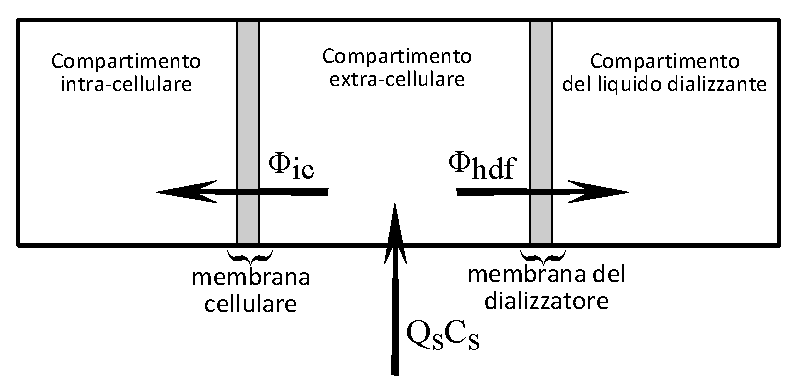
\includegraphics[width=0.8\textwidth]{immagini/massa_ex.eps}
				\caption{Scambio di massa fra compartimento extracellulare, intracellulare e dializzatore.}
\end{figure}
Vale la pena precisare ancora il calcolo di $\Phi_{hdf}$. Dal calcolo teorico esposto in \textsection~\ref{sec:HDF}, risulta:
\begin{multline}\label{eq:phihdf}
		\qquad \Phi_{hdf} = (1-FF)\cdot \biggl[D\bigl(\alpha_d C_{in} - C_d\bigr)+\Phi_t \biggr] + \ldots \\
		                 + FF\cdot \biggl[Q_{in}-(1-\eta)Q_f\biggr] C_{in} \qquad
\end{multline}
col termine convettivo pari a:
\begin{equation*}
	\Phi_t = Q_f \bigl(1-\sigma\bigr) \frac{C_{in} + C_d}{2}
\end{equation*}
Si ricordi che $FF$ è la frazione di filtrazione, pari al rapporto $Q_f/Q_{in}$ fra acqua filtrata e acqua in ingresso al dializzatore. Il calcolo dei coefficienti $D$, $\alpha_d$, $\sigma$ è affrontato in Appendice \ref{app:B}. I valori di concentrazione $C_d$ dei soluti nel liquido di dialisi sono forniti dall'Eq.~(\ref{eq:liquido}).

\subsection{Bilancio di fuidi nel compartimento intra-cellulare}
La variazione nel tempo del volume intracellulare, dipende, attraverso il coefficiente $K_f$ (permeabilità della membrana cellulare all'acqua), dalla differenza osmotica fra spazio intracellulare e spazio interstiziale. In formule:
\begin{equation}\label{eq:vicnot}
	\begin{split}
	\frac{dV_{ic}}{dt} &= Q_{ic}\\
										 &= \gamma K_f \cdot \Delta Osm \\
	                   &= \gamma K_f \sum_j{\sigma_j\biggl(C_{ic}^{(j)}-C_{is}^{(j)}\biggr)}
	\end{split}
\end{equation}
\begin{figure}[htb]
	\centering
		\includegraphics[width=0.5\textwidth]{immagini/vol_ic.eps}
				\caption{Scambio di fluido fra cellule e interstizio.}
\end{figure}
in cui $\gamma=0,93$ è il coefficiente di correzione che tiene conto dell'interazione osmotica fra i soluti; $\sigma_j$ è il coefficiente di riflessione della membrana cellulare nei confronti del soluto $j$ (ricordiamo che l'effetto osmotico è dovuto ai soluti che \textit{non} passano la membrana).
In condizioni di equilibrio, e cioè qualora si sostituissero alle concentrazioni intracellulari e interstiziali dell'Eq.~(\ref{eq:vicnot}) gli opportuni valori ricavati dalla \tablename~\ref{tab:osmolarit} in Appendice \ref{app:A}, si dovrebbe ottenere, per definizione di ``condizione di equilibrio'', che la variazione temporale del volume intracellulare si annulli. Così come è scritta, l'Eq.~(\ref{eq:vicnot}) non soddisfa questa condizione. Ciò è dovuto al fatto di non aver considerato, nella sommatoria, tutti i soluti presenti nell'organismo, solo parte dei quali è tabulata in \tablename~\ref{tab:osmolarit}. Ovviamente è impossibile, data la loro numerosità, considerarli tutti. Ciò non toglie che comunque, nel calcolo dei flussi osmotici, si generi
involontariamente un disequilibrio causato dai soluti mancanti all'appello. Per risolvere questo problema si è pensato di ipotizzare che ogni soluto, in maniera indipendente dagli altri, tenda asintoticamente verso un proprio stato di equilibrio in cui non vi sia più alcun tipo di variazione dinamica, ovvero verso uno stato in cui tutte le derivate temporali che lo riguardano sono nulle.
%, utilizzando un approccio \textit{teleologico}
%\footnote{\textit{`` [\ldots] in fisiologia la dottrina teleologica risulta indubbiamente utile; anche se è ufficialmente respinta, i pericoli che %comporta la sua adozione sono assai modesti [\ldots] ''}.Tratto da A.~C.~Burton, Fisiologia e Biofisica della Circolazione.}, 
%Quando si prendono in considerazione i soluti che interessa analizzare, indipendentemente dalla loro numerosità, ci saranno sempre degli altri soluti, %esclusi dal calcolo, che \textit{all'equilibrio} (ovvero \textit{asintoticamente}) ne bilanceranno l'attività osmotica in quantità pari in modulo a %quella dei soluti inclusi nel calcolo. In altre parole, nel momento in cui i soluti di interesse raggiungeranno lo stato di equilibrio potremmo %ipotizzare che quelli esclusi dal calcolo siano distribuiti in maniera tale che il sistema smetta di evolvere.

A questo punto, è doveroso fare un breve \textit{excursus} per precisare cosa intendiamo, quantitativamente, per ``stato di equilibrio''. In questa trattazione si è deciso di definire come stato di equilibrio quello stato, calcolato ad ogni iterazione, in cui le concentrazioni plasmatiche, interstiziali e intracellulari, abbiano fra loro \textit{gli stessi rapporti numerici} di quelli di \tablename~\ref{tab:osmolarit}. Analogamente, definiamo i \textit{volumi di equilibrio} quei volumi plasmatici, interstiziali e intracellulari, che hanno fra loro \textit{gli stessi rapporti numerici} di quelli in \tablename~\ref{tab:volumi_guyton}. Precisiamo che queste quantità di equilibrio, che il sistema asintoticamente tende a raggiungere, devono essere ricalcolate ad ogni iterazione.

Per ricavare i volumi asintotici di equilibrio, ad ogni iterazione si eseguirà il seguente algoritmo di calcolo:
\begin{align}
		V_{tot,\infty}      &= V_{ic}+V_{is}+V_{pl}   \qquad \text{con $V_{ic}$, $V_{is}$, $V_{pl}$, valori correnti}\\
		V_{pl,\infty}       &= 3/42  \cdot V_{tot,\infty} \\
		V_{is,\infty}       &= 11/42 \cdot V_{tot,\infty} \\
		V_{ic,\infty}       &= 28/42 \cdot V_{tot,\infty} \\
\end{align}
Per ricavare le concentrazioni asintotiche:
\begin{align*}
		M_{tot,\infty} &= M_{ic}+M_{ex} \qquad\qquad \text{con $M_{ic}$, $M_{ex}$, valori correnti}\\
		                     &= V_{pl,\infty}\cdot C_{pl,\infty} + V_{is,\infty}\cdot C_{is,\infty}  + V_{ic,\infty}\cdot C_{ic,\infty} \\
		                     &= V_{pl,\infty}\cdot C_{pl,\infty} + V_{is,\infty}\cdot\alpha_d C_{pl,\infty}  + V_{ic,\infty}\cdot\alpha_d\beta C_{pl,\infty}   \\
		                     &= C_{pl,\infty} \biggl(V_{pl,\infty} + \alpha_d\bigl(V_{is,\infty} + \beta V_{ic,\infty}\bigr)\biggr)
\end{align*}
da cui si ricava:
\begin{align}
		C_{pl,\infty} &= \frac{M_{ic}+M_{ex}}{V_{pl,\infty} + \alpha_d\bigl(V_{is,\infty} + \beta V_{ic,\infty}\bigr)} \\
		C_{is,\infty} &= \alpha_d C_{pl,\infty} \\
		C_{ic,\infty} &= \beta  C_{is,\infty} 
\end{align}
\newline
\indent
Si torni ora ad occuparsi dell'equazione che descrive la variazione del volume intracellulare. Alla luce di tutte le considerazioni fatte sin ora, è possibile costruire il termine \textit{differenza osmotica asintotica} nel seguente modo:
\begin{equation}
	\Delta Osm_{\infty} = \sum_j{\sigma_j\bigl(C_{ic,\infty}^{(j)}-C_{is,\infty}^{(j)}\bigr)}
\end{equation}
Affinché l'Eq.~(\ref{eq:vicnot}) con la quale si è partiti possa soddisfare la condizione che una volta inseriti valori di equilibrio la derivata temporale si annulli in un tempo finito, deve essere modificata e assumere la seguente forma:
\begin{equation}\label{eq:vicyes}
	\begin{split}
	\frac{dV_{ic}}{dt} &= Q_{ic}\\
										 &= \gamma K_f \bigl(\Delta Osm - \Delta Osm_{\infty}\bigr)
	\end{split}										 
\end{equation}
che esplicitata diventa:
\begin{equation*}
	\frac{dV_{ic}}{dt} = \gamma K_f \biggl(\sum_j{\sigma_j\bigl(C_{ic}^{(j)}-C_{is}^{(j)}\bigr)} - \sum_j{\sigma_j\bigl(C_{ic,\infty}^{(j)}-C_{is,\infty}^{(j)}\bigr)}\biggr)
\end{equation*}

\subsection{Bilancio di fluidi nel compartimento interstiziale}
La variazione nel tempo del volume interstiziale dipende sia dalla portata $Q_{ic}$ di liquido che dall'interstizio passa nel compartimento intracellulare, sia dalla portata $Q_{fc}$ di liquido che filtra, attraverso le pareti capillari, dal compartimento plasmatico. Quantitativamente:
\begin{equation}
	\frac{dV_{is}}{dt} = - Q_{ic} + Q_{fc}
\end{equation}
\begin{figure}[htb]
	\centering
		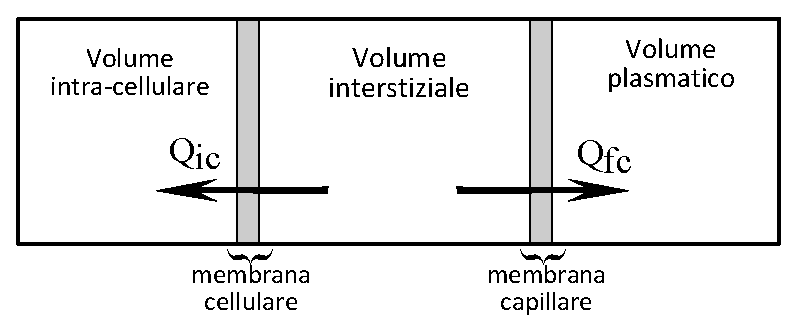
\includegraphics[width=0.8\textwidth]{immagini/vol_is.eps}
				\caption{Scambio di fluidi fra plasma, interstizio e cellule.}
\end{figure}
la portata $Q_{ic}$ si ricava dall'Eq.~(\ref{eq:vicyes}). Per quanto riguarda la portata di filtrazione capillare, essa dipende dalla permeabilità della membrana capillare e dalla differenza di pressione cui è sottoposta. In formule:
\begin{equation}\label{eq:qfcnot}
	Q_{fc} = \rho(L_a+L_v)\cdot P_{fc}
\end{equation}
I parametri $L_a$ e $L_v$ rappresentano rispettivamente le permeabilità nella zona arteriosa e venosa della membrana capillare\footnote{questi elementi sono in parallelo fra loro e, poiché la premeabilità idraulica è analoga alla conduttanza elettrica, la premeabilità/conduttanza totale di due elementi posti in parallelo è data dalla somma delle singole permeabilità/conduttanze.}; il parametro adimensionale $\rho$ serve a dare variabilità alla permeabilità dei capillari, in quanto questa varia da paziente a paziente in base a comorbidità quali diabete, stato infiammatorio, \ldots
La pressione di filtrazione $P_{fc}$ dipende dalla pressione idraulica media nel letto capillare, dalla pressione idraulica dell'interstizio, e dalla differenza di pressione oncotica fra plasma e interstizio, cioè:
\begin{equation}
	P_{fc} = \biggl(\frac{P_{ac}+P_{vc}}{2} - P_{is}\biggr) - \Delta \Pi
\end{equation}
in cui la differenza di pressione oncotica $\Delta \Pi$ è calcolata con la formula di Landis-Pappenheimer in base alla concentrazione proteica dei rispettivi compartimenti. Le pressioni idrauliche si calcolano a partire dai volumi, attraverso i valori di \textit{compliance} o \textit{elastanza} dei relativi compartimenti:
\begin{align}
  P_{is} &= E_{is} (V_{is}-V_{is,0}) + P_{is,0} \qquad \text{con $E_{is}=$ elastanza dell'interstizio}\\
	P_{ac} &= \frac{1}{Cc} (V_{pl}-V_{pl,0}) + P_{is,0} \qquad \text{con $C_c=$ compliance capillare} \\
	P_{vc} &= 15\text{ mmHg} \qquad \text{costante}
\end{align}

Se ora si dà nuovamente uno sguardo al riquadro ``paziente'' di \figurename\ref{schema_generale}, si nota che è stato tralasciato un importante dettaglio di bilancio fra plasma e interstizio: il sistema linfatico. Il sistema linfatico, quando non è compromesso da particolari patologie, svolge l'importante funzione di regolare il bilancio di fluidi fra plasma e interstizio favorendo, ad esempio in caso di edema interstiziale, lo spostamento di liquidi e proteine dall'interstizio al plasma \cite{guyton}. Per tenere in considerazione anche il sistema linfatico si ipotizza che la sua funzione possa essere identificata da una pressione \textit{efficace}, che bilancia la pressione di filtrazione capillare $P_{fc}$. Questa pressione efficace è pari, in modulo, alla pressione di filtrazione capillare quando questa è calcolata utilizzando i valori asintotici di equilibrio, cioè:
\begin{equation}
	P_{fc,\infty} = \biggl(\frac{1/C_c\cdot V_{pl,\infty} + P_{vc}}{2} - E_{is}\cdot V_{is,\infty}\biggr) - \Delta \Pi_{\infty}
\end{equation}
Con quanto appena esposto, l'Eq.~(\ref{eq:qfcnot}) diventa:
\begin{equation}\label{eq:qfcyes}
	Q_{fc} =  \rho\cdot\bigl(L_a+L_v\bigr) \bigl(P_{fc}-P_{fc,\infty}\bigr)
\end{equation}
ed effettuando le sostituizioni opportune, la variazione nel tempo del volume interstiziale è descritta dall'equazione:
\begin{equation}\label{eq:dVis}
	\frac{dV_{is}}{dt} = - \gamma K_f \bigl(\Delta Osm - \Delta Osm_{\infty}\bigr) + \rho \bigl(L_a+L_v\bigr)\cdot \bigl(P_{fc}-P_{fc,\infty}\bigr)
\end{equation}


\subsection{Bilancio di fluidi nel compartimento plasmatico}
La variazione nel tempo del volume plasmatico è descritta dall'equazione:
\begin{equation}\label{eq:dVpl}
	\frac{dV_{pl}}{dt} = -Q_{fc} - Q_{uf}
\end{equation}
\begin{figure}[htb]
	\centering
		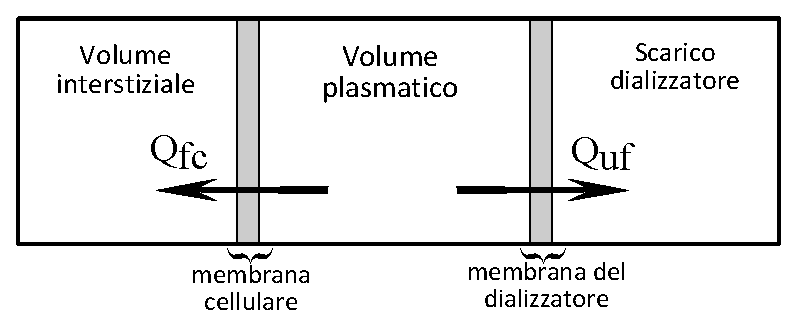
\includegraphics[width=0.8\textwidth]{immagini/vol_dia.eps}
				\caption{Scambio di fluido fra interstizio, plasma e dializzatore.}
\end{figure}
in cui $Q_{fc}$ è dato dall'Eq.~(\ref{eq:qfcyes}); $Q_{uf}$ è la portata di ultrafiltrazione, cioè la portata che permette la perdita di peso del paziente durante la seduta dialitica. Bisogna fare attenzione a non confondere la portata di ultrafiltrazione con la portata di filtrazione del filtro dializzatore. Quest'ultima è infatti data dalla somma di ultrafiltrazione e portata di diluizione. Nell'Eq.~(\ref{eq:dVpl}) non compare la portata di diluizione proprio perché tutto il liquido di diluizione immesso nel circuito ematico viene filtrato dal dializzatore.
